\maketitle

\section{Laboratorio}

Realizar el diseño y simulacion en SIMULINK del codificador y decodificador MLT-3.

\section{Solución}
\subsection{Diseño del codificador}

\begin{figure}[H]
    \centering
    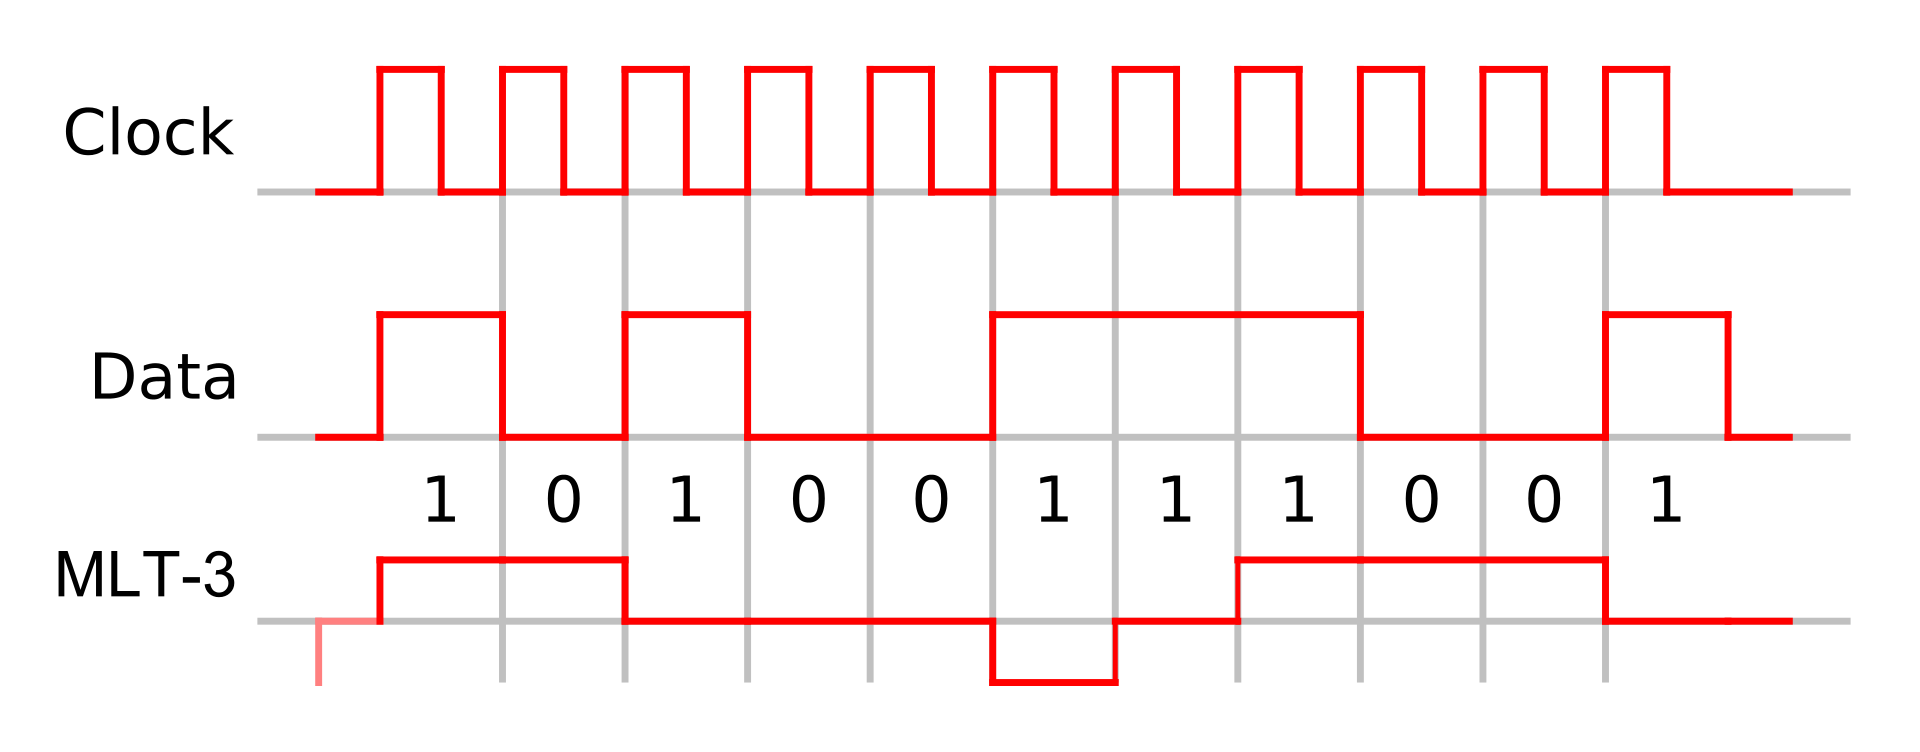
\includegraphics[width=1\textwidth]{laboratorioMLT3/imagenes/MLT3encoding.png}
    \caption{\label{ejemplo}Ejemplo del codificador MLT-3}
\end{figure}

Al analizar el ejemplo de la figura \ref{ejemplo} , se describe que cuando la entrada esta en 0, la salida no presenta cambios, mientras que si esta en 1, la salida cambia entre -1 0 1 dependiendo de su estado anterior, si estaba en -1 o 1, se pasa al estado de 0, mientras que si estaba en 0 se pasa al estado opuesto al ultimo que tuvo, si la señal venia de un -1 ahora pasara a 1 y viseversa. Se explicara mejor el funcionamiento en base al siguiente diagrama de estados de la figura \ref{estados}.

\begin{figure}[H]
    \centering
    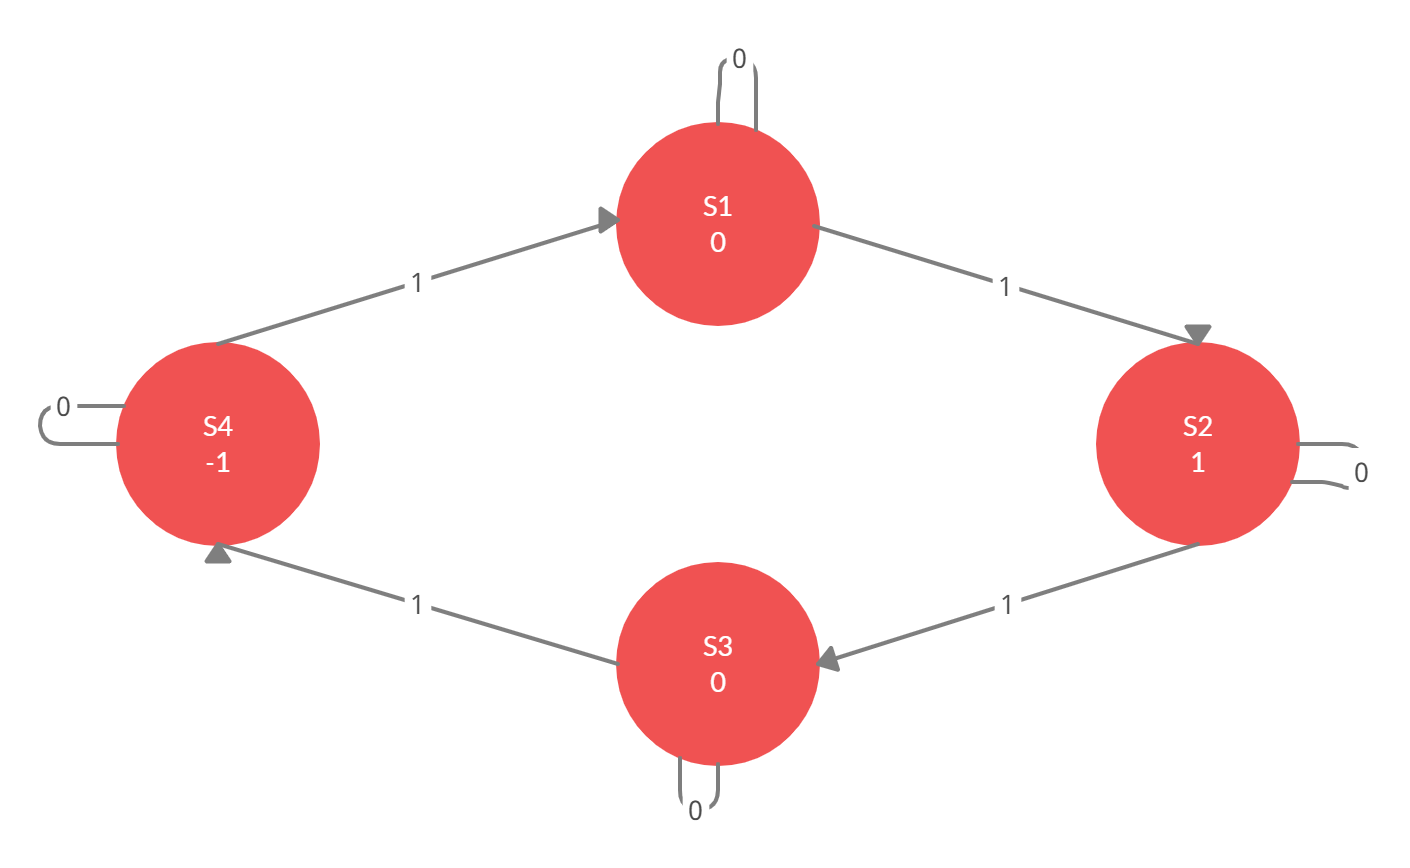
\includegraphics[width=1\textwidth]{laboratorioMLT3/imagenes/Untitled Workspace (1).png}
    \caption{\label{estados}Diagrama de estados}
\end{figure}

Ahora, se especifican las matrices de transicion $T_0$ y $T_1$.
\\
Dado que para entradas en 0 no hay cambios de estado, la matriz de transicion para $T_0$ corresponde a una matriz identidad.

\begin{equation*}
    T_0 = 
    \begin{bmatrix}
        1 & 0 & 0 & 0\\
        0 & 1 & 0 & 0\\
        0 & 0 & 1 & 0\\
        0 & 0 & 0 & 1
    \end{bmatrix}
\end{equation*}

Las entradas en 1 representan cambios al siguiente estado, por lo cual la matriz $T_1$ queda de la forma.

\begin{equation*}
    T_1 = 
    \begin{bmatrix}
        0 & 0 & 0 & 1\\
        1 & 0 & 0 & 0\\
        0 & 1 & 0 & 0\\
        0 & 0 & 1 & 0
    \end{bmatrix}
\end{equation*}

Ya con estas matrices, se procede a implementar la ecuacion de transicion de estados.

\begin{equation*}
    s_{k+1}=[a_{k+1}^*T_0+a_{k+1}T_1]s_k
\end{equation*}

Donde $a_{k+1}$ es la informacion de entrada. $s_k$ viene dada por la siguiente ecuacion.

\begin{equation*}
    s_k = 
    \begin{bmatrix}
        b_k^*e_k^* \\
        b_k^*e_k   \\
        b_ke_k^*   \\
        b_ke_k
    \end{bmatrix}
\end{equation*}

Donde $b_k e_k$ representan los bits de estado del diagrama de estados.\\
Por lo cual la ecuacion de transicion de estados queda de la forma.

\begin{equation*}
    \begin{bmatrix}
        b_{k+1}^*e_{k+1}^* \\
        b_{k+1}^*e_{k+1}   \\
        b_{k+1}e_{k+1}^*   \\
        b_{k+1}e_{k+1}
    \end{bmatrix}
    =
    \left(
    a_{k+1}^*
    \begin{bmatrix}
        1 & 0 & 0 & 0\\
        0 & 1 & 0 & 0\\
        0 & 0 & 1 & 0\\
        0 & 0 & 0 & 1
    \end{bmatrix}
    +
    a_{k+1}
    \begin{bmatrix}
        0 & 0 & 0 & 1\\
        1 & 0 & 0 & 0\\
        0 & 1 & 0 & 0\\
        0 & 0 & 1 & 0
    \end{bmatrix}
    \right)
    \begin{bmatrix}
        b_k^*e_k^* \\
        b_k^*e_k   \\
        b_ke_k^*   \\
        b_ke_k
    \end{bmatrix}
\end{equation*}

Resolviendo las operaciones se obtienen las siguientes cuatro ecuaciones.

\begin{equation}
    \label{eq:1}
    b_{k+1}^*e_{k+1}^*=a_{k+1}^*b_k^*e_k^*+a_{k+1}b_ke_k
\end{equation}

\begin{equation}
    \label{eq:2}
    b_{k+1}^*e_{k+1}=a_{k+1}^*b_k^*e_k+a_{k+1}b_k^*e_k^*=b_k^*(a_{k+1}\oplus e_k)
\end{equation}

\begin{equation}
    \label{eq:3}
    b_{k+1}e_{k+1}^*=a_{k+1}^*b_k e_k^*+a_{k+1}b_k^*e_k
\end{equation}

\begin{equation}
    \label{eq:4}
    b_{k+1}e_{k+1}=a_{k+1}^*b_k e_k+a_{k+1}b_k e_k^*=b_k(a_{k+1}\oplus e_k)
\end{equation}

Ahora se busca obtener el valor de $b_{k+1}$ y $e_{k+1}$, para ello se suman las ecuaciones \ref{eq:3} y \ref{eq:4} lo cual permite obtener la ecuacion de $b_{k+1}$, quedando de la forma.

\begin{equation*}
    b_{k+1}=a_{k+1}^*b_k+a_{k+1}(b_k\oplus e_k)
\end{equation*}

Para obtener la ecuacion de $e_{k+1}$, se suman las ecuaciones \ref{eq:2} y \ref{eq:4}.

\begin{equation*}
    e_{k+1}=a_{k+1}\oplus e_k
\end{equation*}

\subsection{Simulacion del codificador}

Se implementan las ecuaciones del diseño del encoder tal como se muestra en la figura \ref{coder}.

\begin{figure}[H]
    \centering
    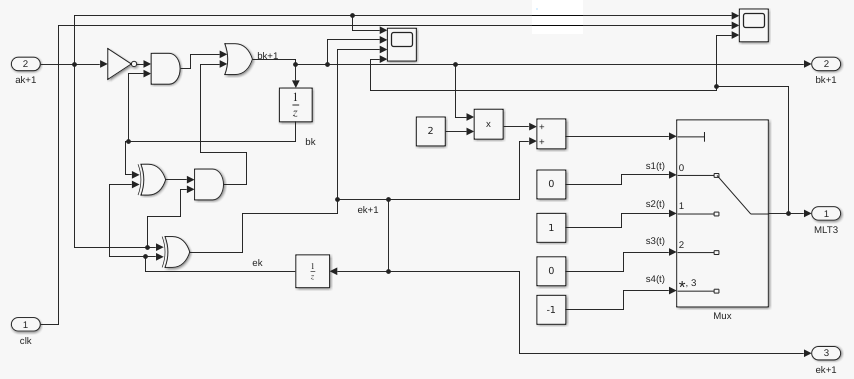
\includegraphics[width=1\textwidth]{laboratorioMLT3/imagenes/coder.PNG}
    \caption{\label{coder}Circuito del codificador}
\end{figure}

Lo cual da la siguiente salida del codificador tal como se ve en la figura \ref{sico}.

\begin{figure}[H]
    \centering
    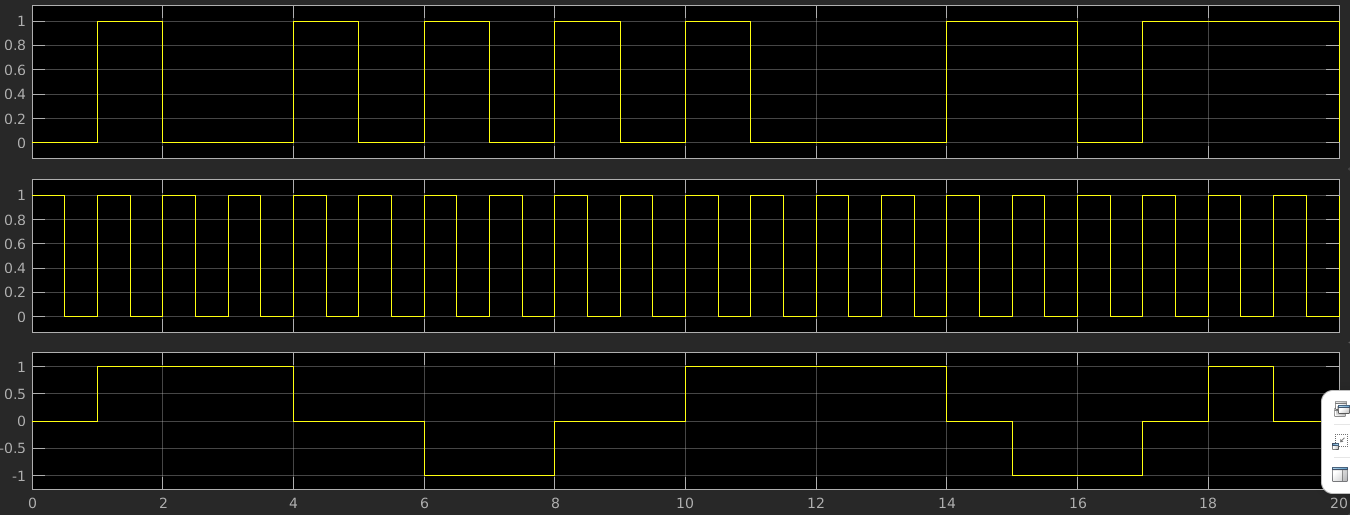
\includegraphics[width=1\textwidth]{laboratorioMLT3/imagenes/simulacionCoder.PNG}
    \caption{\label{sico}Simulacion del codificador}
\end{figure}

La primera grafica corresponde a la señal transmitida, la segunda grafica corresponde al reloj, la tercera es la salida del codificador.

\begin{figure}[H]
    \centering
    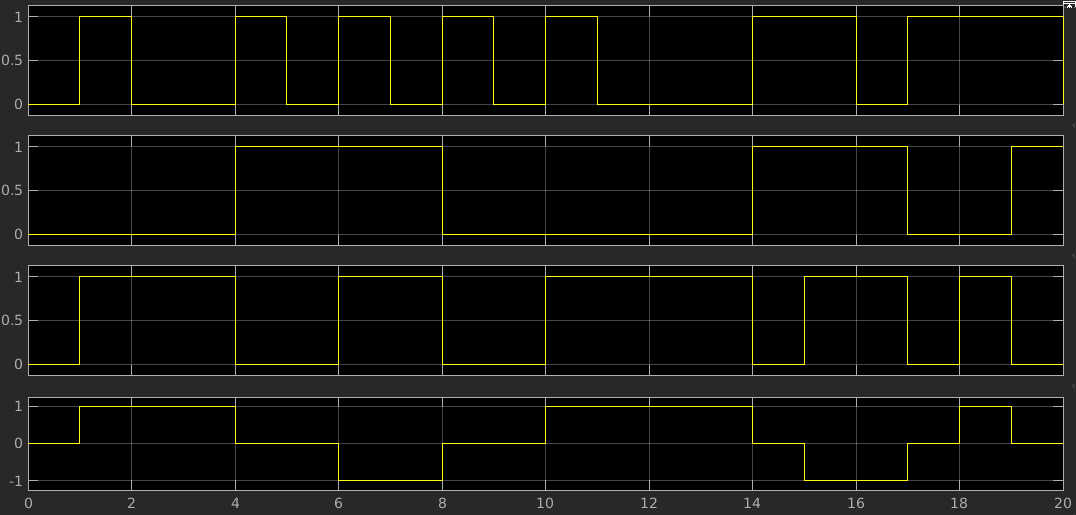
\includegraphics[width=1\textwidth]{laboratorioMLT3/imagenes/simulacionCoder2.PNG}
    \caption{\label{sico2}Simulacion del codificador}
\end{figure}

La figura \ref{sico2} tiene la señal de entrada, la señal $b_{k+1}$ y $e_{k+1}$ que representan las señales de estado, y la señal de salida del codificador.

\subsection{Diseño del decodificador}

Para el diseño del decodificador, se basara en capturar la señal emitida por el codificador y en base a sus estados, se obtendra la señal original de entrada.\\
La figura \ref{deco} explica el funcionamiento de la maquina de estados que permitira decodificar la señal.

\begin{figure}[H]
    \centering
    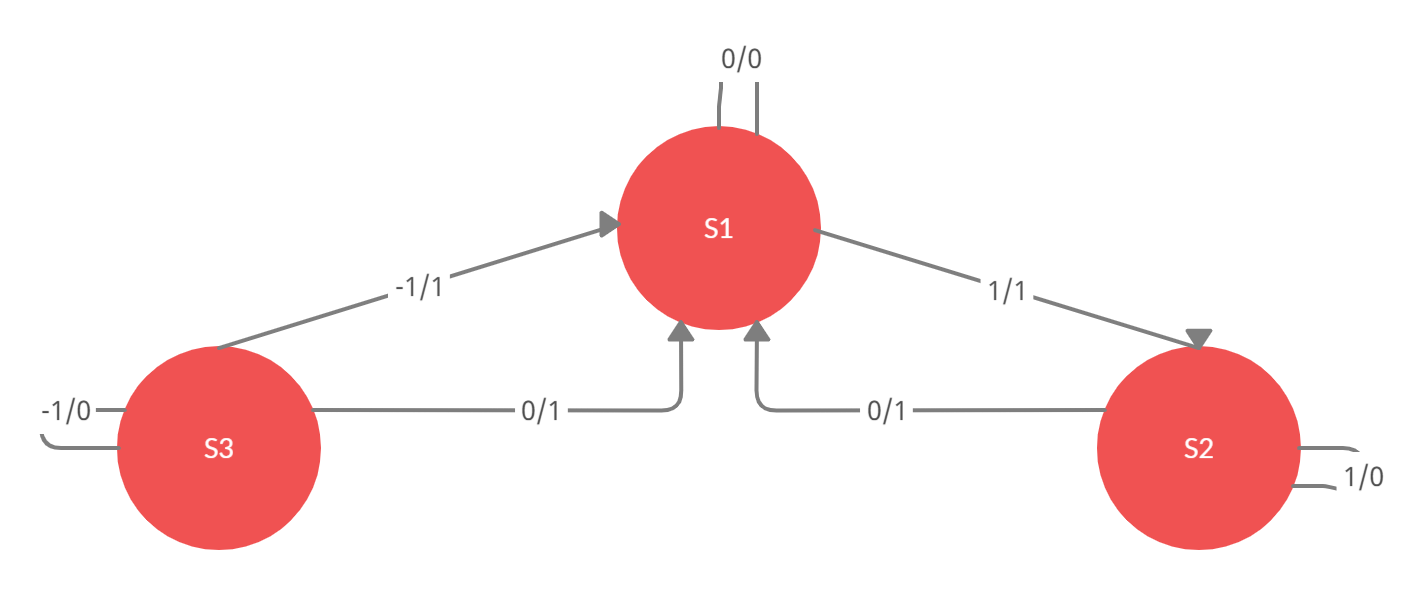
\includegraphics[width=1\textwidth]{laboratorioMLT3/imagenes/Untitled Workspace (2).png}
    \caption{\label{deco}Diagrama de estados del decodificador}
\end{figure}

Donde la salida depende del cambio de estados y permite obtener la señal decodificada.\\
El codificador emite señales con los valores de $0$ $1$ y $-1$, por lo cual el $-1$ se representara como un 2 binario. Ya teniendo una señal binaria, el bit mas significativa va representado por $x_0$ y el menos significativo por $x_1$. La tabla de estados se especifica a continuacion.

\vspace{0.6cm}
\begin{tabular}{| c | c | c | c | c | c | c |}
\hline
 $s_a$ & $s_b$ & $x_0$ & $x_1$ & $s_{a+1}$ & $s_{b+1}$ & $a_{k+1}$\\ \hline
0 & 0 & 0 & 0 & 0 & 0 & 0 \\
0 & 0 & 0 & 1 & 0 & 1 & 1 \\
0 & 0 & 1 & 0 & 1 & 0 & 1 \\
0 & 0 & 1 & 1 & x & x & x \\
0 & 1 & 0 & 0 & 0 & 0 & 1 \\
0 & 1 & 0 & 1 & 0 & 1 & 0 \\
0 & 1 & 1 & 0 & x & x & x \\
0 & 1 & 1 & 1 & x & x & x \\
1 & 0 & 0 & 0 & 0 & 0 & 1 \\
1 & 0 & 0 & 1 & x & x & x \\
1 & 0 & 1 & 0 & 1 & 0 & 0 \\
1 & 0 & 1 & 1 & x & x & x \\
\hline
\end{tabular}
\vspace{0.2cm}

Basados en la tabla anterior, se obtuvieron las siguientes ecuaciones.

\begin{equation*}
    s_{a+1}=x_0
\end{equation*}

\begin{equation*}
    s_{b+1}=x_1
\end{equation*}

\begin{equation}
    \label{eq:deco}
    a_{k+1} = (s_b\oplus x_1)+(s_a\oplus x_0)
\end{equation}

\subsection{Simulacion del decodificador}

Se implementan las ecuaciones obtenidas en el diseño, tal como se muestra en la figura \ref{decoSimu}.

\begin{figure}[H]
    \centering
    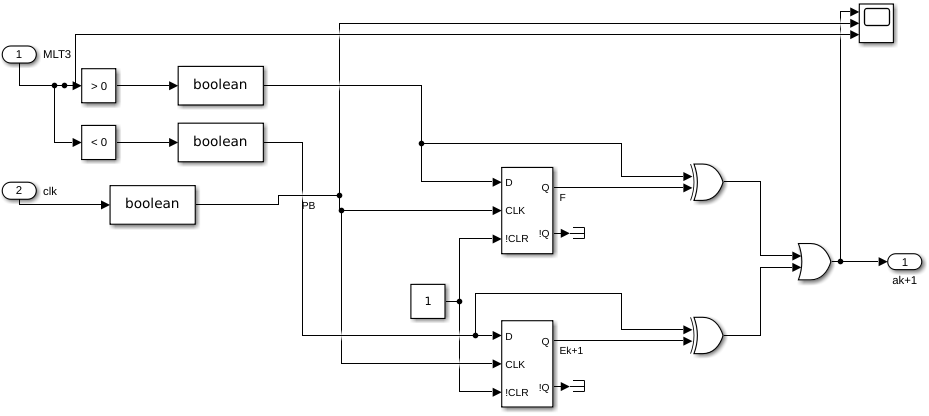
\includegraphics[width=1\textwidth]{laboratorioMLT3/imagenes/decoder.PNG}
    \caption{\label{decoSimu}Circuito del decodificador}
\end{figure}

Primero se transforma la señal del codificador a binario mediante el uso de comparadores que permiten separar cada bit, los cuales se le asignan a cada flip flop tipo D, luego se aplica la ecuacion \ref{eq:deco} para poder obtener la señal decodificada.\\
\\
Se obtiene la siguiente simulacion.

\begin{figure}[H]
    \centering
    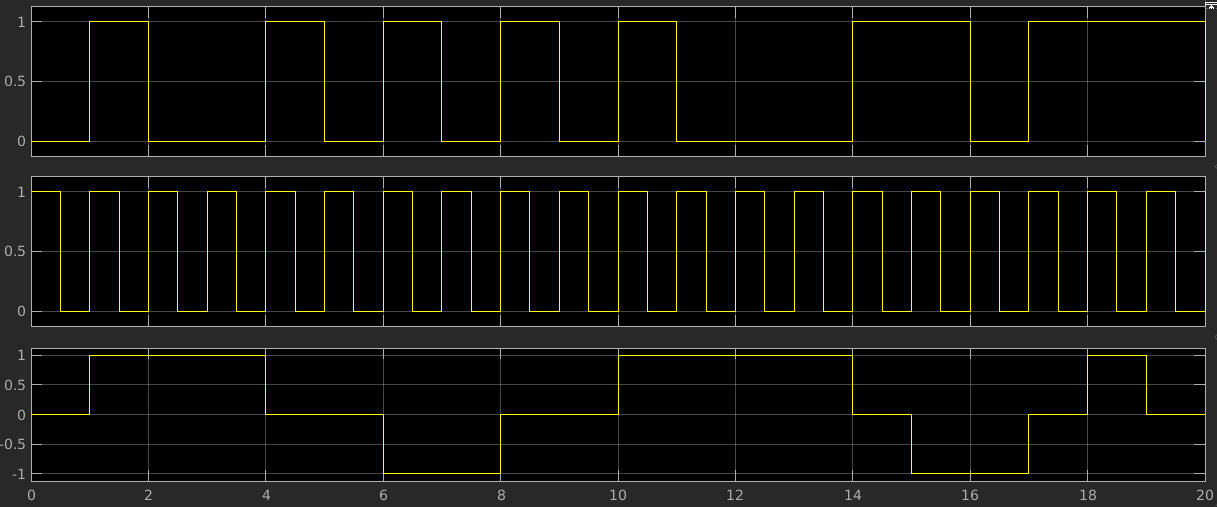
\includegraphics[width=1\textwidth]{laboratorioMLT3/imagenes/simulacionDecoder.PNG}
    \caption{\label{}Simulacion del decoder}
\end{figure}

Donde la primera grafica es la salida del decodificador, la segunda el reloj y la tercera es la entrada del decodificador.

\subsection{Resultados}

Finalmente el circuito queda de la siguiente forma

\begin{figure}[H]
    \centering
    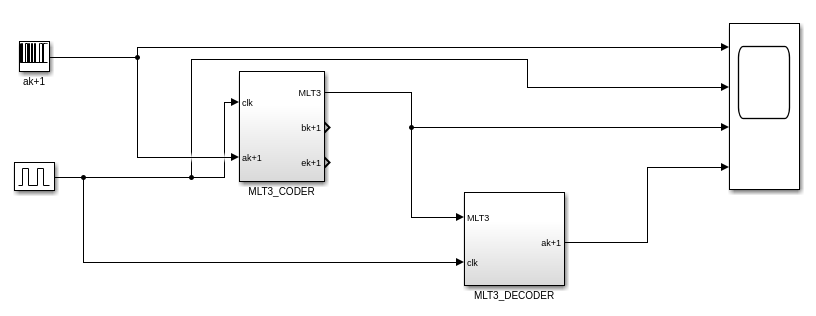
\includegraphics[width=1\textwidth]{laboratorioMLT3/imagenes/circuitoFinal.PNG}
    \caption{\label{}Circuito final}
\end{figure}

Se simula el circuito.

\begin{figure}[H]
    \centering
    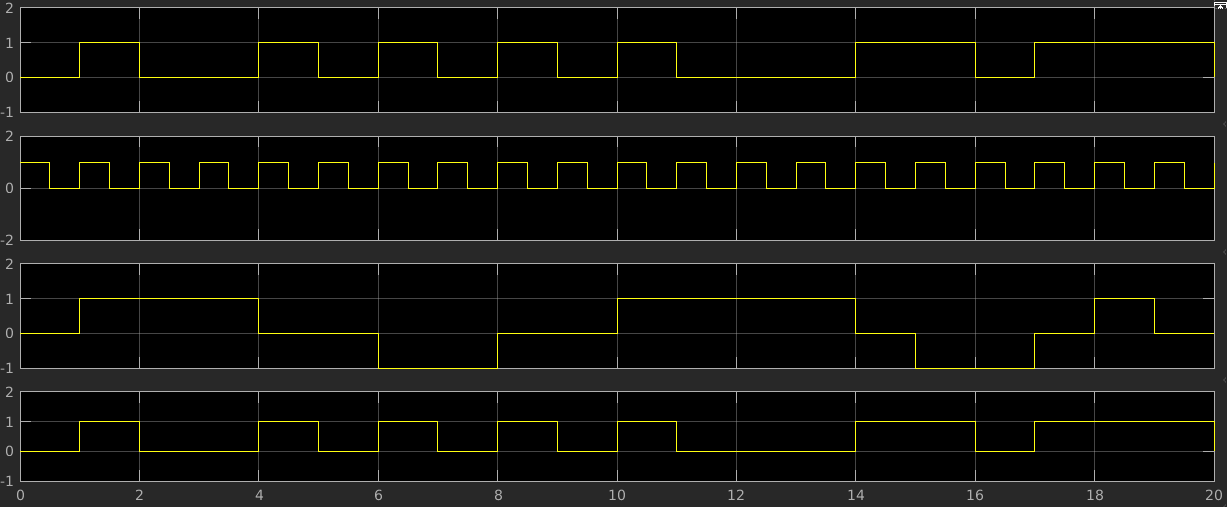
\includegraphics[width=1\textwidth]{laboratorioMLT3/imagenes/simulacionFinal.PNG}
    \caption{\label{}Simulacion final}
\end{figure}

La primera grafica corresponde a la señal a enviar, la segunda el reloj, la tercera es la salida del codificador y la cuarta es la salida del decodificador.